\section{Case Study: eBPF}
\label{sec:analysis}

% In this section, we apply the \emph{\sys} methodology to analyze the evolution and development of the eBPF subsystem in the Linux kernel. Our goal is to uncover insights into the lifecycle, stability, and design decisions of key eBPF features. The survey results are validated through expert review and both quantitative and qualitative analyses.
In this section, we apply the \sys framework designed in Section~\ref{sec:design} to analyze the evolution and development of the eBPF subsystem in the Linux kernel. Our goal is to uncover how different stakeholders perceive the lifecycle, stability, and design decisions of key eBPF features. The multi-agent analysis reveals divergent perspectives that mirror real community dynamics, validated through expert review and consensus metrics.

The Extended Berkeley Packet Filter (eBPF)~\cite{ebpf} is a rapidly evolving subsystem in the Linux kernel that allows users to run sandboxed programs in kernel space without modifying the kernel itself~\cite{lim2024safebpf}. Originally developed for packet filtering, eBPF now supports diverse use cases such as performance tracing, security monitoring, and system observability, and has been expanded to multiple platforms~\cite{windows-ebpf,zheng2023bpftime}. The academic community has identified current problems and limitations of eBPF, proposing several works to improve aspects like the verifier and deployment.

\subsection{Research Questions for Survey Evaluation}

% To ensure that the LLM does not answer questions randomly, we evaluate the effectiveness and correctness of the \emph{\sys} results by exploring the following high-level research questions:
To ensure that our multi-agent framework provides meaningful insights rather than random responses, we evaluate the effectiveness and correctness of the \sys results by exploring the following high-level research questions:

\begin{itemize}
    \item \textbf{Correctness of Survey Responses:} How can we ensure that survey responses reflect accurate and relevant information about the system's features and commits?
    \item \textbf{Consistency Across Similar Questions:} Are similar questions answered consistently across different but related features or subsystems?
    \item \textbf{Coverage of Survey Questions:} Do the survey questions comprehensively cover all relevant aspects of the feature or subsystem under analysis?
    \item \textbf{Insight from Survey:} Can the survey data help users analyze the design, implementation, maintenance, reliability, and security evolution, and gain valuable insights?
    \item \textbf{Clarity and Ambiguity in Responses:} Are the survey responses clear and unambiguous, making them actionable for further analysis?

    \item \textbf{Expert Confirmation:} How do experts rate the accuracy of the survey's generated insights?
\end{itemize}

\subsection{Survey Design and Implementation}

To gain deeper insights into the design and evolution of the eBPF subsystem, we developed a comprehensive survey aimed at classifying commits within the Linux eBPF subsystem. The survey evaluates specific aspects of each commit by analyzing commit messages and associated code changes, with questions covering commit classification, complexity, affected components, and use cases.

\subsection{Implementing the Survey Using LLM Agents}

To efficiently process and analyze the vast number of commits in the Linux eBPF subsystem, we leveraged the \sys framework to instantiate Empirically-Grounded Personas (as described in Section~\ref{sec:design}). Using CrewAI~\cite{crewai}, we created agents representing actual eBPF contributors such as the Alexei Starovoitov agent (eBPF maintainer), Brendan Gregg agent (observability expert), and KP Singh agent (security perspective). Each agent maintains personalized memory systems for their complete contribution history, email threads, and documented design philosophies. By utilizing GPT-4o~\cite{gpt4o} as based model with these memory-enhanced agents, we captured not just technical analysis but the authentic perspectives of real developers. We applied this approach to over 15,000 commits and 150,000+ emails, with agents responding based on their historical positions while revealing genuine disagreements that mirror actual community dynamics.

\subsubsection{Commit Survey Methodology}

Following the workflow described in Section~\ref{sec:design}, each agent analyzes commits through their personalized lens: (1) memory retrieval: the agent searches their RAG-indexed Knowledge Base for similar past commits, related discussions, and previous decisions, (2) contextual analysis: combining the new commit with retrieved memories to form opinions consistent with their historical stance, (3) perspective-based classification: the Alexei Starovoitov agent might flag a verifier change as "high-risk" while the Brendan Gregg agent sees it as "enabling new observability", (4) collaborative review: agents debate classifications in Phase 3 (Asynchronous Community Review), with disagreements revealing real community tensions, and (5) consensus building: the Critic-Resolver agent (Phase 4) captures both majority views and dissenting opinions.

The memory-augmented agents maintain consistency with their real-world counterpart's documented positions while allowing natural evolution of views based on new evidence.

\subsubsection{Enhancing Survey Accuracy}

Accuracy can be enhanced through: multiple survey runs (we ran once due to budget, achieving <1\% error), domain-specific fine-tuning or advanced models like O1~\cite{o1}, clearer prompts, and multi-step processes for complex commits.

LLM automation enabled efficient processing of tens of thousands of commits, transforming unstructured data into structured insights.

% \subsection{The Commit Dataset}

% The \texttt{commit\_survey.csv} dataset provides metadata for over 15,000 Linux kernel commits, including commit types, messages, timestamps, and affected components. It categorizes and classifies commits, focusing on the eBPF subsystem.

% \subsubsection{Dataset Overview}

% The dataset contains the following fields:

% \begin{itemize}
%     \item \textbf{Commit Metadata}: Unique commit IDs, author and committer details, and timestamps.
%     \item \textbf{Commit Messages and File Changes}: Descriptions of the changes in each commit.
%     \item \textbf{Classification}: Types such as bug fixes, feature additions, or merges.
%     \item \textbf{Complexity}: Based on the number of files and lines changed.
%     \item \textbf{Components}: Affected implementation and logic components.
%     \item \textbf{Use Cases}: Related subsystems and modules.
% \end{itemize}

% \subsubsection{Key Findings from Dataset Analysis}

% Our analysis reveals several important patterns in eBPF subsystem development:

% \textbf{Commit Classification:} Most commits focus on bug fixes and code cleanups, reflecting efforts to maintain code quality. Significant attention goes to testing infrastructure changes, emphasizing robustness. New features constitute a considerable portion of commits, while merge commits are commonplace in Linux kernel development.

% \textbf{Commit Complexity:} Most commits are simple, involving small changes, while complex changes constitute a smaller portion. This distribution suggests eBPF development follows an incremental improvement pattern.

% \textbf{Implementation Components:} Test cases and build scripts are significantly affected, highlighting continuous testing and build improvements. The \texttt{libbpf} library is a key component in the kernel eBPF toolchain, receiving considerable attention. Substantial development occurs in other kernel subsystems, particularly eBPF events. Frequent updates to the verifier and helpers indicate efforts to enhance functionality and ensure program safety. Some commits appear unrelated to the eBPF subsystem.

% \textbf{Logic Components:} General utilities, such as tools and scripts, receive the most updates, followed by runtime features like helpers and kernel functions, which are consistently enhanced. eBPF event logic and instruction handling are also frequently updated to ensure robustness and functionality.

% \textbf{Use Cases and Events:} While most commits enhance the core eBPF infrastructure—including the verifier and runtime components—significant development also extends to networking-related features such as socket and XDP programs, which receive substantial attention. Additionally, tracing tools like tracepoints and kprobes highlight eBPF's crucial role in system diagnostics and debugging.


\subsection{Development Artifacts: Commits and Communications}

Our analysis encompasses over 15,000 Linux kernel commits and 150,000+ mailing list emails from the eBPF subsystem, captured in the \texttt{commit\_survey.csv} dataset. This comprehensive dataset includes commit metadata (IDs, authors, timestamps), commit messages and file changes, classification categories (bug fixes, features, merges), complexity metrics based on files and lines changed, affected components (implementation and logic), and related use cases and subsystems. The email corpus provides additional context about design decisions, community discussions, and feature evolution that complements the commit data.

Key findings reveal distinct development patterns: Most commits focus on bug fixes and code cleanups, with significant attention to testing infrastructure, reflecting the community's emphasis on stability and robustness. The complexity distribution shows predominantly simple, incremental changes, characteristic of mature kernel development. Implementation analysis highlights that test cases and build scripts receive the most updates, while the \texttt{libbpf} library receives considerable attention. Frequent updates to the verifier and helpers indicate efforts to enhance functionality and ensure program safety. Notably, some commits appear unrelated to the eBPF subsystem due to broad filtering criteria. For logic components, general utilities receive the most updates, followed by runtime features like helpers and kernel functions. Networking features (socket, XDP) and tracing tools (kprobes, tracepoints) represent major development areas, underscoring eBPF's dual role in both network processing and system observability. The email discussions reveal heated debates around verifier complexity, API stability, and the balance between feature velocity and kernel maintainability—tensions that our multi-agent framework captures through divergent agent perspectives.

\subsection{Correctness of Survey Responses}

To ensure that the survey responses accurately reflect system features and commits, we validated the results by randomly sampling the data and cross-referencing with expert knowledge and processing logs. Specifically, we addressed two common issues: the handling of merge commits and the identification of commits unrelated to the eBPF subsystem.

We observed discrepancies in how merge commits were classified between the commit classification and the major implementation component perspectives. To address this, we analyzed the top merge commit messages and found that some merge commits were categorized based on their predominant effect on a specific component rather than being uniformly labeled as merge commits. By clarifying this distinction in the survey questions, we ensured that the classification system accurately reflected the commit's impact across different perspectives.

\textbf{Example:}
\begin{verbatim}
Top Commit (Classification but not Implementation):
3    Merge branch 'bpf-fix-incorrect-name-check-pass'
25   Merge branch 'vsc73xx-fix-mdio-and-phy' Pawel...
\end{verbatim}

\subsubsection{Non-Related eBPF Subsystem Commits}

We noted that commits not directly related to the eBPF subsystem were sometimes included due to broad filtering criteria (e.g., \texttt{--grep=bpf}). Upon reviewing these commits, we confirmed that some mentioned ``bpf'' but addressed unrelated or peripheral issues.

\textbf{Example:}
\begin{verbatim}
Sample 'Not related to eBPF' Commit Messages:
17    bonding: fix xfrm real_dev null pointer...
21    btrfs: fix invalid mapping of extent xarray st...
\end{verbatim}

\subsubsection{Consistency Across Similar Questions}

We checked for consistency in responses by comparing related questions, focusing on the number of merge commits in commit classifications and complexities, as well as the number of commits unrelated to the eBPF subsystem in the implementation and logic components.

\textbf{Example 1: Merge Commits}
\begin{itemize}
    \item \textbf{Commit Classification:} ``It's like a merge commit.'' (2,130 responses)
    \item \textbf{Commit Complexity:} ``Merge-like. The commit merges branches.'' (2,132 responses)
\end{itemize}

\textbf{Example 2: Unrelated Components}
\begin{itemize}
    \item \textbf{Implementation Component:} ``Not related to eBPF.'' (773 responses)
    \item \textbf{Logic Component:} ``Not related to eBPF.'' (766 responses)
\end{itemize}

The close alignment of these numbers demonstrates consistent identification of unrelated components. With a low misclassification rate (under 0.05\% for total commits), our data shows high consistency, supporting the reliability of the survey design.

\subsection{Timeline Analysis of Commits}

Analyzing the timeline of commits provides valuable insights into the evolution of the eBPF subsystem over time. By visualizing the distribution of commit types, complexities, and major components across different periods, we can identify trends and patterns in the development of eBPF features.

The data was processed by cleaning to remove irrelevant commits, smoothing using a 3-month average to reduce noise and highlight long-term trends, and treating single-component \texttt{Merge} commits as regular commits while removing multi-component \texttt{Merge} commits, such as mainline merges. The time span covers from 2017 to the end of 2024, encompassing over 15,000 commits.

\subsubsection{Commit Classification Over Time}

\begin{figure}[ht]
    \centering
    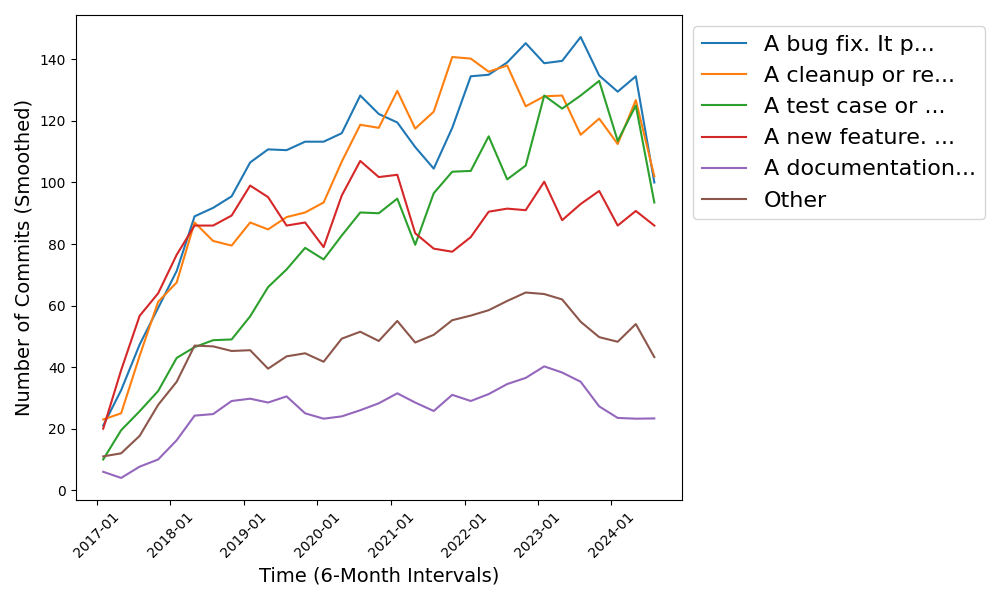
\includegraphics[width=\linewidth]{feature-analysis/timeline_commit_classification_smoothed.png}
    \caption{Commit Classification Over Time}
    \label{fig:timeline_commit_classification_smoothed}
\end{figure}

Figure~\ref{fig:timeline_commit_classification_smoothed} shows the distribution of different types of commits over time.

The development began to grow significantly in 2017, with limited addition of test cases initially, which continued to improve over time. New feature development follows a cyclical pattern, with notable spikes around 2020 and 2021. After 2021, the number of cleanups and refactorings increases significantly, while new feature additions decline, indicating a shift in focus towards code maintainability and stability. A decline in cleanup commits after 2023 suggests that while new features continue to be added, the emphasis has shifted more towards stabilization and optimization.

\subsubsection{Commits Related to Major Implementation Components Over Time}

\begin{figure}[ht]
    \centering
    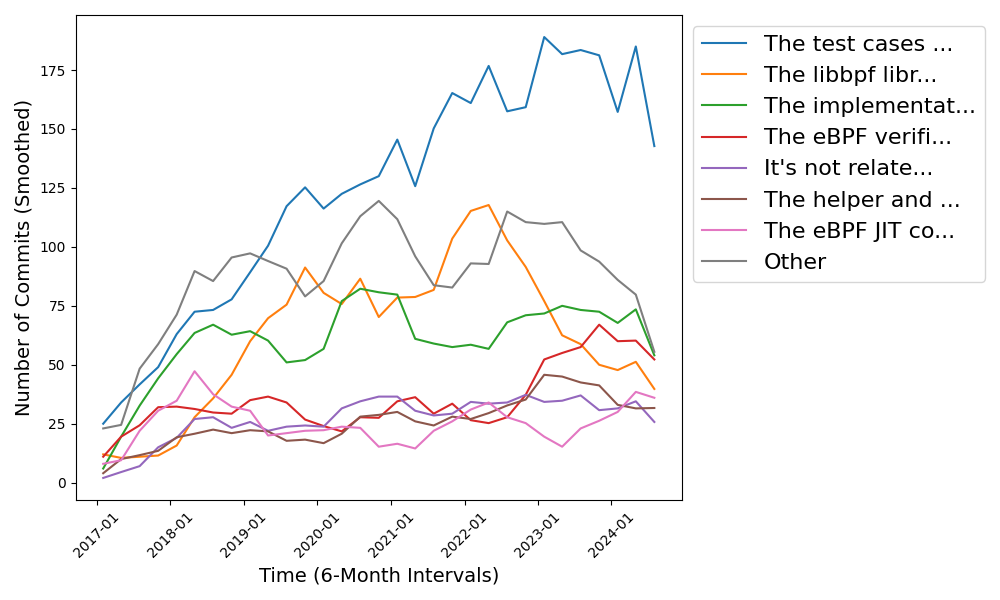
\includegraphics[width=\linewidth]{feature-analysis/timeline_major_related_implementation_component_smoothed.png}
    \caption{Commits Related to Major Implementation Components Over Time}
    \label{fig:timeline_major_related_implementation_component_smoothed}
\end{figure}

Figure~\ref{fig:timeline_major_related_implementation_component_smoothed} illustrates the evolution of major implementation components in the Linux eBPF subsystem.

Most components experienced their highest activity between 2017 and 2022, reflecting the rapid development of eBPF features during this period. The \texttt{libbpf} library saw the most dramatic increase, while the JIT compiler was most frequently updated around 2018. The rise in test cases also reflects the growing importance of a robust testing framework in this field.

After peaking around 2021--2022, several components show a decline or stabilization in activity. This indicates that many eBPF components have entered a phase of optimization and maintenance rather than new feature development, while testing continues to increase coverage. The verifier shows modest activity throughout the observed period but seems to increase in 2023--2024, which may reflect renewed research efforts in this area.

\subsubsection{Commits Related to Major Logic Components Over Time}

\begin{figure}[ht]
    \centering
    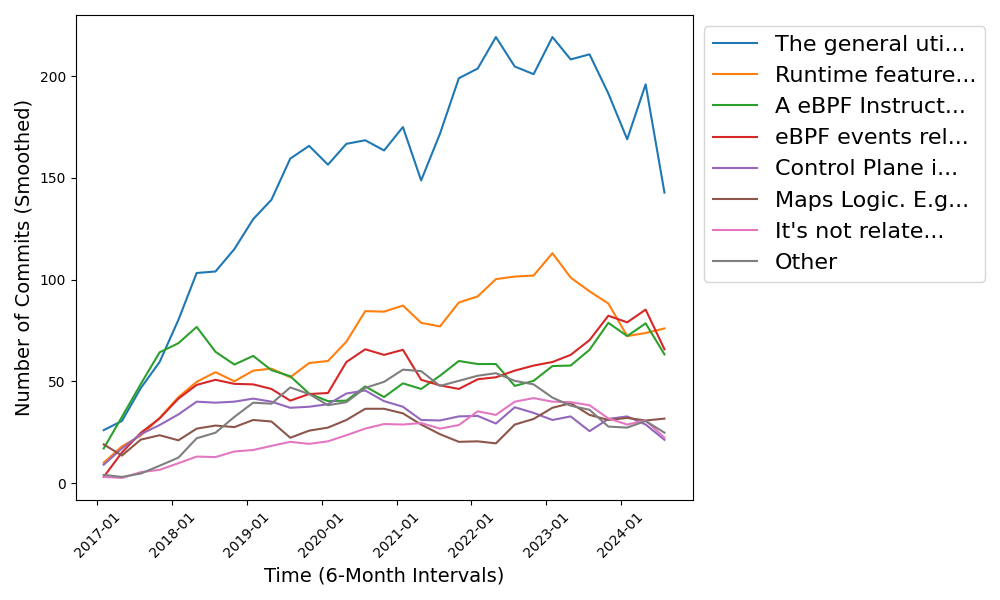
\includegraphics[width=\linewidth]{feature-analysis/timeline_major_related_logic_component_smoothed.png}
    \caption{Commits Related to Major Logic Components Over Time}
    \label{fig:timeline_major_related_logic_component_smoothed}
\end{figure}

Figure~\ref{fig:timeline_major_related_logic_component_smoothed} illustrates the evolution of major logic components within the Linux eBPF subsystem over time. The \texttt{General Utilities} component, which includes test cases and build scripts, exhibits the most significant improvements, reaching a peak between 2022 and 2023 before experiencing a decline. In contrast, the \texttt{eBPF Instruction Logic} component displays two prominent peaks in 2018 and 2024, corresponding to the initial introduction of eBPF instructions and subsequent standardization efforts, respectively.

Other components, such as \texttt{Runtime Features, Helpers, and kfuncs}, show a notable peak in 2023 followed by a decrease and subsequent stabilization. Meanwhile, the \texttt{Control Plane Interface} and \texttt{Maps Logic} components maintain relatively steady levels of activity throughout the observed period.

\subsubsection{Use Cases or Events Over Time}

\begin{figure}[ht]
    \centering
    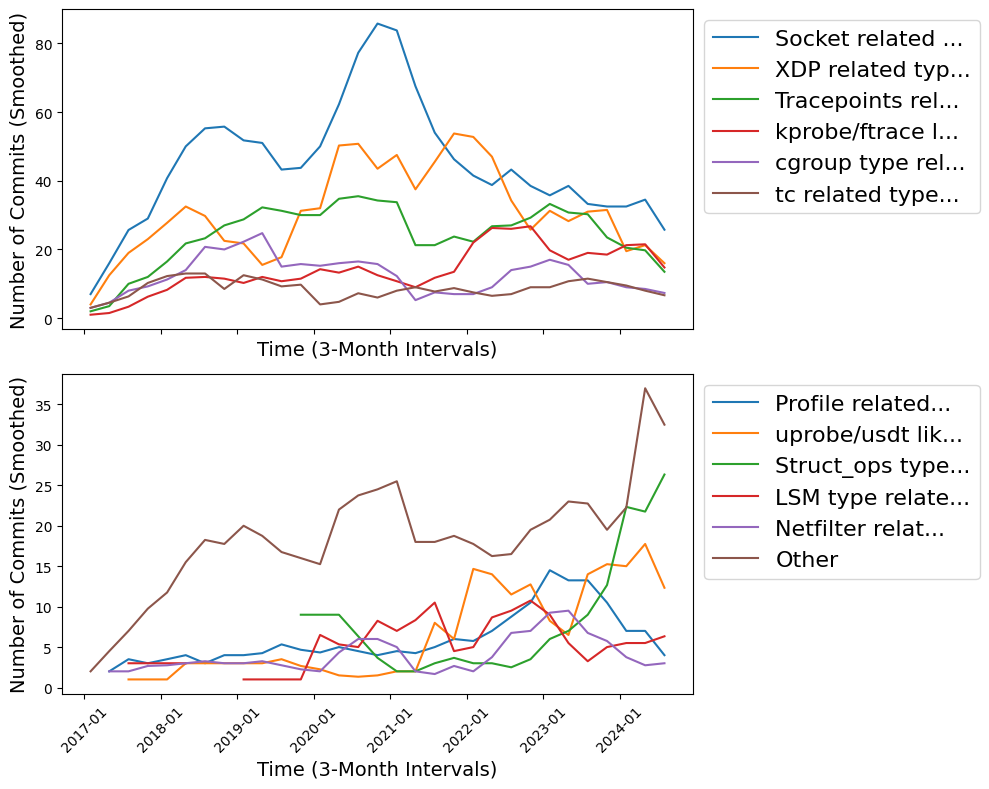
\includegraphics[width=\linewidth]{feature-analysis/timeline_usecases_or_submodule_events_smoothed.png}
    \caption{Use Cases or Events Over Time}
    \label{fig:timeline_usecases_or_submodule_events_smoothed}
\end{figure}

Figure~\ref{fig:timeline_usecases_or_submodule_events_smoothed} reveals significant fluctuations in event types over the years.

Notably, network-related events such as socket and XDP programs experienced a surge from 2020 to 2022, after which they entered a stabilization phase following the initial burst of feature additions and optimizations. The tracepoints-related activities show a steady increase with periodic fluctuations, peaking around 2021 before decreasing. The kprobe/ftrace-related events remain mostly stable, with a slight increase in 2022. Uprobe-related events show moderate activity over several years, with slight peaks in 2022 and again in 2024. The \texttt{struct\_ops}, an emerging feature introduced in 2020, shows a significant increase in activity between 2023 and 2024. Other events such as LSM for security remain minor.

\subsection{Deeper Insights Analysis}

This section delves into the survey responses to uncover patterns, trends, and areas for improvement within the eBPF subsystem.

\subsubsection{Which Kernel Components and Files Have the Most Frequent Bugs?}

\begin{figure}[ht]
    \centering
    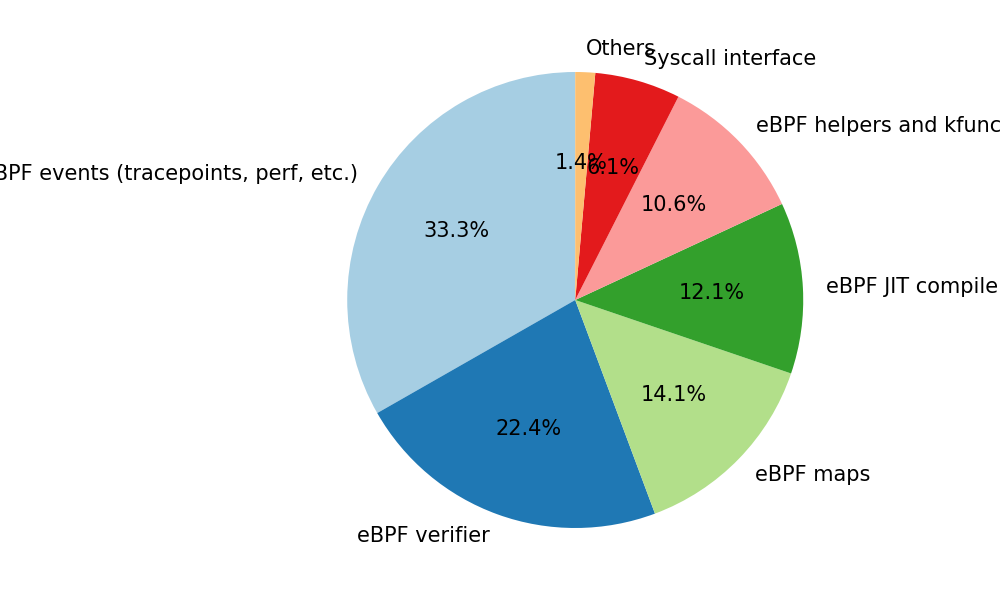
\includegraphics[width=\linewidth]{feature-analysis/kernel_components_most_buggy_pie_chart.png}
    \caption{Kernel Implementation Components with the Most Bugs}
    \label{fig:buggy_kernel_component}
\end{figure}

Figure~\ref{fig:buggy_kernel_component} illustrates the kernel implementation components with a high number of bugs. While previous analyses and tools have primarily focused on improving the stability of the verifier and JIT compiler, these areas account for only about 35\% of the bugs. The largest number of bugs originate from eBPF event-related code, which involves the interaction of eBPF with other kernel subsystems. Additionally, helpers and maps also have a significant number of bugs. Due to the complexity of the control plane, the eBPF syscall interface is also prone to bugs.

By examining specific files, we observe that bugs frequently occur in the verifier, syscall, core, and network filter components. These files require better test coverage and more attention.

\textbf{Top 10 Buggy Files:}
\begin{verbatim}
kernel/bpf/verifier.c             425
net/core/filter.c                 140
kernel/bpf/syscall.c              111
include/linux/bpf.h                87
kernel/bpf/core.c                  83
include/uapi/linux/bpf.h           80
kernel/trace/bpf_trace.c           77
kernel/bpf/btf.c                   75
tools/include/uapi/linux/bpf.h     54
kernel/bpf/sockmap.c               51
\end{verbatim}

\subsubsection{What is the Relationship Between Instruction-Related Changes in the Verifier and All Verifier Bugs?}

\begin{figure}[ht]
    \centering
    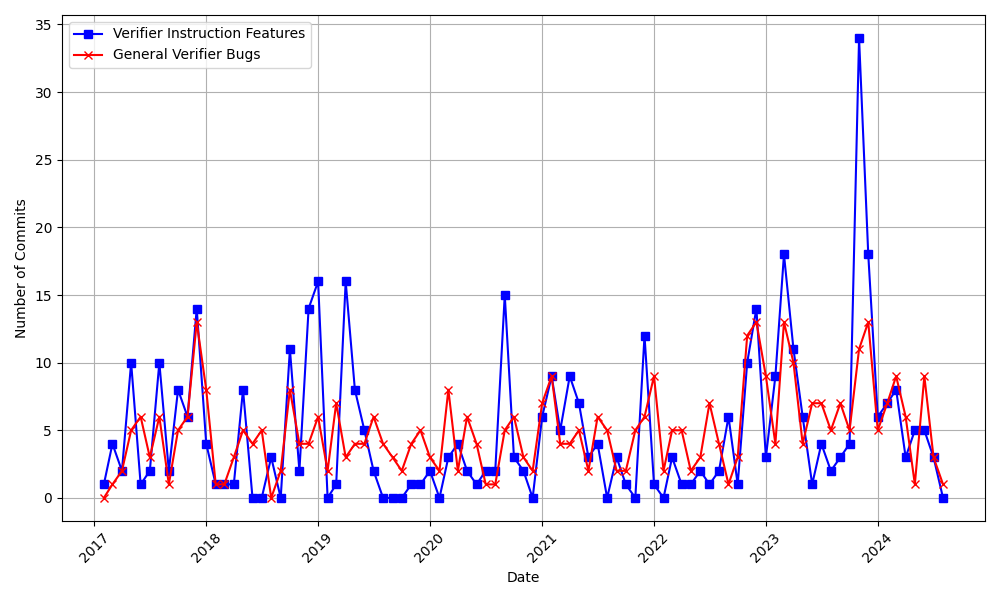
\includegraphics[width=\linewidth]{feature-analysis/verifier_features_vs_general_bugs_over_time.png}
    \caption{Verifier Bugs or Features Related to eBPF Instructions Over Time}
    \label{fig:instruction_verifier_features_bugs_over_time}
\end{figure}

Figure~\ref{fig:instruction_verifier_features_bugs_over_time} shows that changes related to eBPF instructions in the verifier closely correlate with the number of verifier bugs. This insight highlights the importance of focusing on instruction-related aspects during verifier development and debugging to enhance overall system stability.

\subsubsection{The Evolution and Status of \texttt{libbpf}}

We also examined the lifecycle of specific components, such as \texttt{libbpf}.

Based on Figure~\ref{fig:libbpf_commit_classification}, the development of \texttt{libbpf} began to grow significantly in 2017. New feature development follows a cyclical pattern, with notable spikes around 2020 and 2022. After 2022, the number of cleanups and refactorings increased significantly, indicating a shift in focus towards code maintainability and stability. However, the decline in cleanup commits after 2023 suggests that while new features continue to be added, the emphasis has shifted more towards stabilization and optimization.

Historical milestones verify this trend. For instance, \texttt{libbpf} version 1.0 was released in August 2022~\cite{libbpf1}, and the major feature ``Compile Once, Run Everywhere'' (CO-RE) was introduced around 2020~\cite{core}, both aligning with the peaks and shifts observed in the commit history.

\begin{figure}[ht]
    \centering
    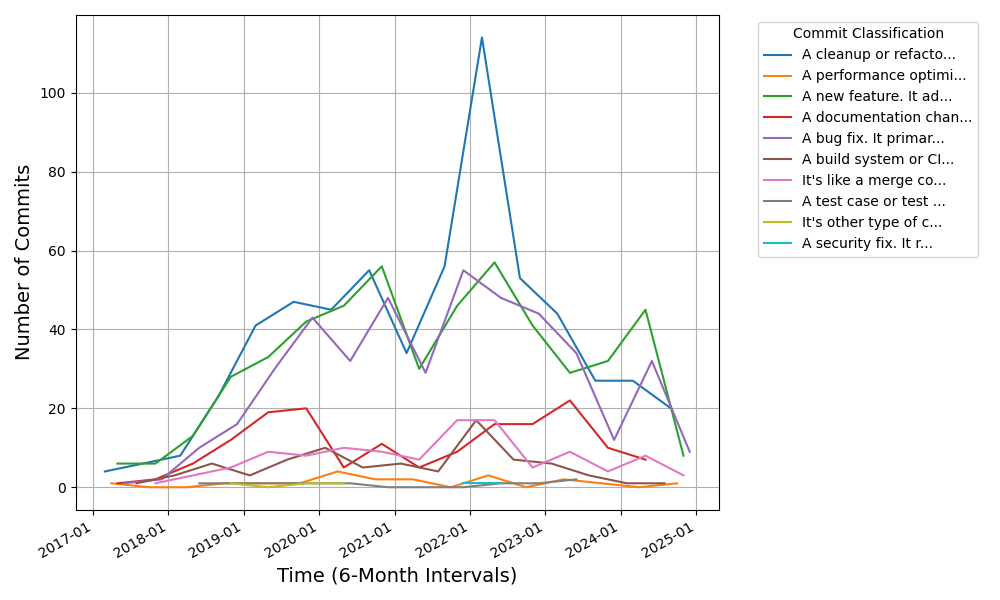
\includegraphics[width=\linewidth]{feature-analysis/libbpf_evolution_by_classification.png}
    \caption{Evolution of \texttt{libbpf} Over Time}
    \label{fig:libbpf_commit_classification}
\end{figure}

\subsubsection{What Dependencies Have Emerged Between Features and Components?}

Our analysis of feature-component dependencies in Figure~\ref{fig:feature_component_heatmap} reveals two primary patterns. First, new control plane abstractions such as \texttt{bpf\_link}\cite{bpflink} and \texttt{token}\cite{token} typically require coordinated updates to both the \texttt{syscall interface} and \texttt{libbpf}, indicating tightly coupled development. Second, runtime features like \texttt{bpf\_iter}\cite{bpf_iterators} and \texttt{spin\_lock}\cite{spinlock} mainly depend on internal kernel components such as \texttt{helpers} and \texttt{verifier}, with minimal impact on the \texttt{JIT compiler}, suggesting potential areas for JIT optimization.


\begin{figure}[ht]
    \centering
    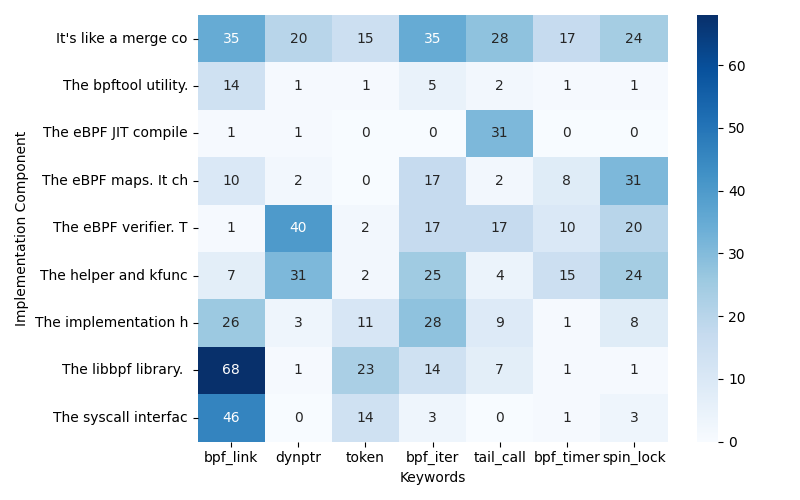
\includegraphics[width=\linewidth]{feature-analysis/heatmap_bpf_keywords_vs_components.png}
    \caption{Feature-Component Interdependencies in the BPF Subsystem}
    \label{fig:feature_component_heatmap}
\end{figure}


\subsection{Survey Validation}

% To validate the effectiveness of \sys, we employed multiple approaches. First, we discussed the results with more than five eBPF experts who have submitted kernel patches or presented at conferences; they confirmed that the findings align with their understanding of eBPF evolution. We also shared the report with kernel maintainers and the BPF kernel mailing list for broader validation. Second, the survey responses proved to be generally clear and actionable, with minimal ambiguity in the structured data extracted from commits. Third, by comparing survey responses with real-world feature changes and historical milestones (such as the release of libbpf 1.0 and the introduction of CO-RE), we confirmed that the survey accurately captures the historical context of eBPF development. The consistency between our automated analysis and expert knowledge demonstrates that \sys can effectively transform unstructured development artifacts into reliable, structured insights about software evolution.
To validate the effectiveness of \sys and verify that it achieves the design goals outlined in Section~\ref{sec:design}, we employed multiple approaches. First, we discussed the multi-agent results with more than five eBPF experts who confirmed that the agent disagreements mirror real community tensions: maintainers indeed prioritize stability while contributors push features. We also shared the report with kernel maintainers and the BPF kernel mailing list, who validated that our virtual community accurately reflects real dynamics. Second, the multi-perspective responses revealed nuanced insights, with inter-agent disagreements highlighting genuine areas of community debate. Third, by comparing agent consensus patterns with real-world feature controversies (such as the BPF type format debates and verifier complexity discussions), we confirmed that \sys captures not just technical evolution but social dynamics. The correlation between agent disagreements and actual mailing list debates demonstrates that \sys effectively models how different stakeholders perceive kernel evolution, providing insights into collaboration patterns crucial for the FM era.

% \bibliographystyle{IEEEtran}
% \bibliography{references}